% -*- Mode:TeX -*-

%% IMPORTANT: The official thesis specifications are available at:
%%            http://libraries.mit.edu/archives/thesis-specs/
%%
%%            Please verify your thesis' formatting and copyright
%%            assignment before submission.  If you notice any
%%            discrepancies between these templates and the 
%%            MIT Libraries' specs, please let us know
%%            by e-mailing thesis@mit.edu

%% The documentclass options along with the pagestyle can be used to generate
%% a technical report, a draft copy, or a regular thesis.  You may need to
%% re-specify the pagestyle after you \include  cover.tex.  For more
%% information, see the first few lines of mitthesis.cls. 

%\documentclass[12pt,vi,twoside]{mitthesis}
%%
%%  If you want your thesis copyright to you instead of MIT, use the
%%  ``vi'' option, as above.
%%
%\documentclass[12pt,twoside,leftblank]{mitthesis}
%%
%% If you want blank pages before new chapters to be labelled ``This
%% Page Intentionally Left Blank'', use the ``leftblank'' option, as
%% above. 

\documentclass[12pt,twoside]{mitthesis}
\usepackage{lgrind}
\usepackage[utf8]{inputenc}
\usepackage{amssymb}
%% These have been added at the request of the MIT Libraries, because
%% some PDF conversions mess up the ligatures.  -LB, 1/22/2014
\usepackage{cmap}
\usepackage{amsmath}
\usepackage[T1]{fontenc}
\pagestyle{plain}
\usepackage[hypcap]{caption}
\newcommand{\R}{\mathbb{R}}
%% This bit allows you to either specify only the files which you wish to
%% process, or `all' to process all files which you \include.
%% Krishna Sethuraman (1990).

%\typein [\files]{'chap1'}
\def\all{all}
%\ifx\files\all \typeout{Including all files.} \else \typeout{Including only \files.} \includeonly{\files} \fi

\begin{document}
\pagestyle{plain}


%%% This file is for producing a Doctoral Thesis proposal.  It should be fairly
%% self-explanatory.  

\documentclass{article}
\begin{document}
\bibliographystyle{plain}
\pagestyle{empty}
\markboth{{\sc Projet fil rouge : }}{{\sc Projet fil rouge}}

\def\title{}
\def\author{}
\def\addrone{}
\def\addrtwo{}

\def\degree{}
%% Added \deptname for PhD proposals in other fields.
%% Krishna Sethuraman (1990)
\def\deptname{}
\def\laboratory{}

\def\submissiondate{\today}
\def\completiondate{}

\def\supervisor{}
\def\supertitleone{}
\def\supertitletwo{ }

\def\readerone{Professor ?}
\def\readeronetitleone{Professor ??}
\def\readeronetitletwo{}

\def\readertwo{Professor ??}
\def\readertwotitleone{??}
\def\readertwotitletwo{}

\def\readerthree{Professor ??}
\def\readerthreetitleone{??}
\def\readerthreetitletwo{}


\def\abstract{
\newpage 

\paragraph{}



\paragraph{} 



\paragraph{} 
.

}

%%%%%%%%%%%%%%%%%%%%%%%%%%%%%%%%%%%%%%%%%%%%%%%%%%%%%%%%%%%%%%%%%%%%%%%%%%%%
%%%%%%%%%% You Should Not Need To Modify Anything Below Here %%%%%%%%%%%%%%%
%%%%%%%%%%%%%%%%%%%%%%%%%%%%%%%%%%%%%%%%%%%%%%%%%%%%%%%%%%%%%%%%%%%%%%%%%%%%

%%%%%%%%%%%%%%%%%%%%%%%%%%%%%%%%%
%%% Cover Page - Author signs %%%
%%%%%%%%%%%%%%%%%%%%%%%%%%%%%%%%%

\begin{center}

\end{center}

\vspace{.5in}

\def\sig{{\small \sc (Signature of Author)}}

\begin{tabular}{rlc}
   {\small \sc Title:}                       & \multicolumn{2}{l}{\title}
\\ {\small \sc Submitted by:}
                            & \author  & \\
                            & \addrone & \\
                            & \addrtwo & \\ \cline{3-3}
			    &	       & \makebox[2in][c]{\sig}
\\ {\small \sc Date of Submission:}          & \multicolumn{2}{l}{\submissiondate}
\\ {\small \sc Expected Date of Completion:} & \multicolumn{2}{l}{\completiondate}
\\ {\small \sc Laboratory:}                  & \multicolumn{2}{l}{\laboratory}
\end{tabular}


\vspace{.75in}
{\bf \sc Brief Statement of the Problem:}

\abstract

         %%%%%%%%%%%%%%%%%%%%%%%%%%%%%
\newpage %%% Supervision Agreement %%%
         %%%%%%%%%%%%%%%%%%%%%%%%%%%%%

\begin{flushright}
   Faculty of physics
\\ Department of \deptname
\\ Warsaw
\end{flushright}

\underline{\bf }

\vspace{.25in}
\begin{tabular}{rl}
   {\small \sc To:}   & 
\\ {\small \sc From:} & \supervisor
\end{tabular}

\vspace{.25in}
The program outlined in the proposal:

\vspace{.25in}
\begin{tabular}{rl}
   {\small \sc Title:}  & \title
\\ {\small \sc Author:} & \author
\\ {\small \sc Date:}   & \submissiondate
\end{tabular}

\vspace{.25in}
is adequate for a Doctoral thesis.
I believe that appropriate readers for this thesis would be:

\vspace{.25in}
\begin{tabular}{rl}
   {\small \sc Reader 1:} & \readerone
\\ {\small \sc Reader 2:} & \readertwo
%\\ {\small \sc Reader 3:} & \readerthree
\end{tabular}

\vspace{.25in}


\vspace{.25in}
\begin{tabular}{crc}
  \hspace{2in} & {\sc Signed:} & \\ \cline{3-3}
               &               & {\small \sc \supertitleone} \\
               &               & {\small \sc \supertitletwo} \\
               &               &                             \\
               & {\sc Date:}   & \\ \cline{3-3}
\end{tabular}

\vspace{0in plus 1fill}

Comments: \\
\begin{tabular}{c}
  \hspace{6.25in} \\
  \mbox{} \\ \cline{1-1} \mbox{} \\
  \mbox{} \\ \cline{1-1} \mbox{} \\
  \mbox{} \\ \cline{1-1} \mbox{} \\
%  \mbox{} \\ \cline{1-1} \mbox{} \\
%  \mbox{} \\ \cline{1-1} \mbox{} \\
%  \mbox{} \\ \cline{1-1} \mbox{} \\
\end{tabular}

          %%%%%%%%%%%%%%%%%%%%%%%%%%
\newpage  %%% Reader I Agreement %%%
          %%%%%%%%%%%%%%%%%%%%%%%%%%

\begin{flushright}
   Faculty of physics
\\ Department of \deptname
\\ Warsaw
\end{flushright}

\underline{\bf Doctoral Thesis Reader Agreement}

\vspace{.25in}
\begin{tabular}{rl}
   {\small \sc To:}   & Department Graduate Committee
\\ {\small \sc From:} & \readerone
\end{tabular}

\vspace{.25in}
The program outlined in the proposal:

\vspace{.25in}
\begin{tabular}{rl}
   {\small \sc Title:}          & \title
\\ {\small \sc Author:}         & \author
\\ {\small \sc Date:}           & \submissiondate
\\ {\small \sc Supervisor:}     & \supervisor
\\ {\small \sc Other Reader:}   & \readertwo
%\\ {\small \sc Other Reader:}   & \readerthree
\end{tabular}

\vspace{.25in}
is adequate for a Doctoral thesis.
I am willing to aid in guiding the research
and in evaluating the thesis report as a reader.

\vspace{.25in}
\begin{tabular}{crc}
  \hspace{2in} & {\sc Signed:} & \\ \cline{3-3}
               &               & {\small \sc \readeronetitleone} \\
               &               & {\small \sc \readeronetitletwo} \\
               &               &                                 \\
               & {\sc Date:}   & \\ \cline{3-3}
\end{tabular}

\vspace{0in plus 1fill}

Comments: \\
\begin{tabular}{c}
  \hspace{6.25in} \\
  \mbox{} \\ \cline{1-1} \mbox{} \\
  \mbox{} \\ \cline{1-1} \mbox{} \\
  \mbox{} \\ \cline{1-1} \mbox{} \\
  \mbox{} \\ \cline{1-1} \mbox{} \\
  \mbox{} \\ \cline{1-1} \mbox{} \\
  \mbox{} \\ \cline{1-1} \mbox{} \\
\end{tabular}


          %%%%%%%%%%%%%%%%%%%%%%%%%%%
\newpage  %%% Reader II Agreement %%%
          %%%%%%%%%%%%%%%%%%%%%%%%%%%


\begin{flushright}
   

\end{flushright}

\underline{\bf Projet Fil Rouge}

\vspace{.25in}
\begin{tabular}{rl}
   {\small \sc To:}   & Department Graduate Committee
\\ {\small \sc From:} & \readertwo
\end{tabular}

\vspace{.25in}
The program outlined in the proposal:

\vspace{.25in}
\begin{tabular}{rl}
   {\small \sc Title:}          & \title
\\ {\small \sc Author:}         & \author
\\ {\small \sc Date:}           & \submissiondate
\\ {\small \sc Supervisor:}     & \supervisor
\\ {\small \sc Other Reader:}   & \readerone
%\\ {\small \sc Other Reader:}   & \readerthree
\end{tabular}

\vspace{.25in}
is adequate for a Doctoral thesis.
I am willing to aid in guiding the research
and in evaluating the thesis report as a reader.

\vspace{.25in}
\begin{tabular}{crc}
  \hspace{2in} & {\sc Signed:} & \\ \cline{3-3}
               &               & {\small \sc \readertwotitleone} \\
               &               & {\small \sc \readertwotitletwo} \\
               &               &                                 \\
               & {\sc Date:}   & \\ \cline{3-3}
\end{tabular}

\vspace{0in plus 1fill}

Comments: \\
\begin{tabular}{c}
  \hspace{6.25in} \\
  \mbox{} \\ \cline{1-1} \mbox{} \\
  \mbox{} \\ \cline{1-1} \mbox{} \\
  \mbox{} \\ \cline{1-1} \mbox{} \\
  \mbox{} \\ \cline{1-1} \mbox{} \\
  \mbox{} \\ \cline{1-1} \mbox{} \\
  \mbox{} \\ \cline{1-1} \mbox{} \\
\end{tabular}
\newpage
          %%%%%%%%%%%%%%%%%%%%%%%%%%%
\newpage  %%% Reader III Agreement %%%
          %%%%%%%%%%%%%%%%%%%%%%%%%%%


\begin{flushright}
   Faculty of physics
\\ Department of \deptname
\\ Warsaw
\end{flushright}

\underline{\bf Doctoral Thesis Reader Agreement}

\vspace{.25in}
\begin{tabular}{rl}
   {\small \sc To:}   & Department Graduate Committee
\\ {\small \sc From:} & \readerthree
\end{tabular}

\vspace{.25in}
The program outlined in the proposal:

\vspace{.25in}
\begin{tabular}{rl}
   {\small \sc Title:}          & \title
\\ {\small \sc Author:}         & \author
\\ {\small \sc Date:}           & \submissiondate
\\ {\small \sc Supervisor:}     & \supervisor
\\ {\small \sc Other Reader:}   & \readerone
\\ {\small \sc Other Reader:}   & \readertwo
\end{tabular}

\vspace{.25in}
is adequate for a Doctoral thesis.
I am willing to aid in guiding the research
and in evaluating the thesis report as a reader.

\vspace{.25in}
\begin{tabular}{crc}
  \hspace{2in} & {\sc Signed:} & \\ \cline{3-3}
               &               & {\small \sc \readerthreetitleone} \\
               &               & {\small \sc \readerthreetitletwo} \\
               &               &                                 \\
               & {\sc Date:}   & \\ \cline{3-3}
\end{tabular}

\vspace{0in plus 1fill}

Comments: \\
\begin{tabular}{c}
  \hspace{6.25in} \\
  \mbox{} \\ \cline{1-1} \mbox{} \\
  \mbox{} \\ \cline{1-1} \mbox{} \\
  \mbox{} \\ \cline{1-1} \mbox{} \\
  \mbox{} \\ \cline{1-1} \mbox{} \\
  \mbox{} \\ \cline{1-1} \mbox{} \\
  \mbox{} \\ \cline{1-1} \mbox{} \\
\end{tabular}
\newpage

\end{document}





\include{contents}
% Some departments (e.g. 5) require an additional signature page.  See
% signature.tex for more information and uncomment the following line if
% applicable.
% \include{signature}
%%% This file is for producing a Doctoral Thesis proposal.  It should be fairly
%% self-explanatory.  

\documentclass{article}
\begin{document}
\bibliographystyle{plain}
\pagestyle{empty}
\markboth{{\sc Projet fil rouge : }}{{\sc Projet fil rouge}}

\def\title{}
\def\author{}
\def\addrone{}
\def\addrtwo{}

\def\degree{}
%% Added \deptname for PhD proposals in other fields.
%% Krishna Sethuraman (1990)
\def\deptname{}
\def\laboratory{}

\def\submissiondate{\today}
\def\completiondate{}

\def\supervisor{}
\def\supertitleone{}
\def\supertitletwo{ }

\def\readerone{Professor ?}
\def\readeronetitleone{Professor ??}
\def\readeronetitletwo{}

\def\readertwo{Professor ??}
\def\readertwotitleone{??}
\def\readertwotitletwo{}

\def\readerthree{Professor ??}
\def\readerthreetitleone{??}
\def\readerthreetitletwo{}


\def\abstract{
\newpage 

\paragraph{}



\paragraph{} 



\paragraph{} 
.

}

%%%%%%%%%%%%%%%%%%%%%%%%%%%%%%%%%%%%%%%%%%%%%%%%%%%%%%%%%%%%%%%%%%%%%%%%%%%%
%%%%%%%%%% You Should Not Need To Modify Anything Below Here %%%%%%%%%%%%%%%
%%%%%%%%%%%%%%%%%%%%%%%%%%%%%%%%%%%%%%%%%%%%%%%%%%%%%%%%%%%%%%%%%%%%%%%%%%%%

%%%%%%%%%%%%%%%%%%%%%%%%%%%%%%%%%
%%% Cover Page - Author signs %%%
%%%%%%%%%%%%%%%%%%%%%%%%%%%%%%%%%

\begin{center}

\end{center}

\vspace{.5in}

\def\sig{{\small \sc (Signature of Author)}}

\begin{tabular}{rlc}
   {\small \sc Title:}                       & \multicolumn{2}{l}{\title}
\\ {\small \sc Submitted by:}
                            & \author  & \\
                            & \addrone & \\
                            & \addrtwo & \\ \cline{3-3}
			    &	       & \makebox[2in][c]{\sig}
\\ {\small \sc Date of Submission:}          & \multicolumn{2}{l}{\submissiondate}
\\ {\small \sc Expected Date of Completion:} & \multicolumn{2}{l}{\completiondate}
\\ {\small \sc Laboratory:}                  & \multicolumn{2}{l}{\laboratory}
\end{tabular}


\vspace{.75in}
{\bf \sc Brief Statement of the Problem:}

\abstract

         %%%%%%%%%%%%%%%%%%%%%%%%%%%%%
\newpage %%% Supervision Agreement %%%
         %%%%%%%%%%%%%%%%%%%%%%%%%%%%%

\begin{flushright}
   Faculty of physics
\\ Department of \deptname
\\ Warsaw
\end{flushright}

\underline{\bf }

\vspace{.25in}
\begin{tabular}{rl}
   {\small \sc To:}   & 
\\ {\small \sc From:} & \supervisor
\end{tabular}

\vspace{.25in}
The program outlined in the proposal:

\vspace{.25in}
\begin{tabular}{rl}
   {\small \sc Title:}  & \title
\\ {\small \sc Author:} & \author
\\ {\small \sc Date:}   & \submissiondate
\end{tabular}

\vspace{.25in}
is adequate for a Doctoral thesis.
I believe that appropriate readers for this thesis would be:

\vspace{.25in}
\begin{tabular}{rl}
   {\small \sc Reader 1:} & \readerone
\\ {\small \sc Reader 2:} & \readertwo
%\\ {\small \sc Reader 3:} & \readerthree
\end{tabular}

\vspace{.25in}


\vspace{.25in}
\begin{tabular}{crc}
  \hspace{2in} & {\sc Signed:} & \\ \cline{3-3}
               &               & {\small \sc \supertitleone} \\
               &               & {\small \sc \supertitletwo} \\
               &               &                             \\
               & {\sc Date:}   & \\ \cline{3-3}
\end{tabular}

\vspace{0in plus 1fill}

Comments: \\
\begin{tabular}{c}
  \hspace{6.25in} \\
  \mbox{} \\ \cline{1-1} \mbox{} \\
  \mbox{} \\ \cline{1-1} \mbox{} \\
  \mbox{} \\ \cline{1-1} \mbox{} \\
%  \mbox{} \\ \cline{1-1} \mbox{} \\
%  \mbox{} \\ \cline{1-1} \mbox{} \\
%  \mbox{} \\ \cline{1-1} \mbox{} \\
\end{tabular}

          %%%%%%%%%%%%%%%%%%%%%%%%%%
\newpage  %%% Reader I Agreement %%%
          %%%%%%%%%%%%%%%%%%%%%%%%%%

\begin{flushright}
   Faculty of physics
\\ Department of \deptname
\\ Warsaw
\end{flushright}

\underline{\bf Doctoral Thesis Reader Agreement}

\vspace{.25in}
\begin{tabular}{rl}
   {\small \sc To:}   & Department Graduate Committee
\\ {\small \sc From:} & \readerone
\end{tabular}

\vspace{.25in}
The program outlined in the proposal:

\vspace{.25in}
\begin{tabular}{rl}
   {\small \sc Title:}          & \title
\\ {\small \sc Author:}         & \author
\\ {\small \sc Date:}           & \submissiondate
\\ {\small \sc Supervisor:}     & \supervisor
\\ {\small \sc Other Reader:}   & \readertwo
%\\ {\small \sc Other Reader:}   & \readerthree
\end{tabular}

\vspace{.25in}
is adequate for a Doctoral thesis.
I am willing to aid in guiding the research
and in evaluating the thesis report as a reader.

\vspace{.25in}
\begin{tabular}{crc}
  \hspace{2in} & {\sc Signed:} & \\ \cline{3-3}
               &               & {\small \sc \readeronetitleone} \\
               &               & {\small \sc \readeronetitletwo} \\
               &               &                                 \\
               & {\sc Date:}   & \\ \cline{3-3}
\end{tabular}

\vspace{0in plus 1fill}

Comments: \\
\begin{tabular}{c}
  \hspace{6.25in} \\
  \mbox{} \\ \cline{1-1} \mbox{} \\
  \mbox{} \\ \cline{1-1} \mbox{} \\
  \mbox{} \\ \cline{1-1} \mbox{} \\
  \mbox{} \\ \cline{1-1} \mbox{} \\
  \mbox{} \\ \cline{1-1} \mbox{} \\
  \mbox{} \\ \cline{1-1} \mbox{} \\
\end{tabular}


          %%%%%%%%%%%%%%%%%%%%%%%%%%%
\newpage  %%% Reader II Agreement %%%
          %%%%%%%%%%%%%%%%%%%%%%%%%%%


\begin{flushright}
   

\end{flushright}

\underline{\bf Projet Fil Rouge}

\vspace{.25in}
\begin{tabular}{rl}
   {\small \sc To:}   & Department Graduate Committee
\\ {\small \sc From:} & \readertwo
\end{tabular}

\vspace{.25in}
The program outlined in the proposal:

\vspace{.25in}
\begin{tabular}{rl}
   {\small \sc Title:}          & \title
\\ {\small \sc Author:}         & \author
\\ {\small \sc Date:}           & \submissiondate
\\ {\small \sc Supervisor:}     & \supervisor
\\ {\small \sc Other Reader:}   & \readerone
%\\ {\small \sc Other Reader:}   & \readerthree
\end{tabular}

\vspace{.25in}
is adequate for a Doctoral thesis.
I am willing to aid in guiding the research
and in evaluating the thesis report as a reader.

\vspace{.25in}
\begin{tabular}{crc}
  \hspace{2in} & {\sc Signed:} & \\ \cline{3-3}
               &               & {\small \sc \readertwotitleone} \\
               &               & {\small \sc \readertwotitletwo} \\
               &               &                                 \\
               & {\sc Date:}   & \\ \cline{3-3}
\end{tabular}

\vspace{0in plus 1fill}

Comments: \\
\begin{tabular}{c}
  \hspace{6.25in} \\
  \mbox{} \\ \cline{1-1} \mbox{} \\
  \mbox{} \\ \cline{1-1} \mbox{} \\
  \mbox{} \\ \cline{1-1} \mbox{} \\
  \mbox{} \\ \cline{1-1} \mbox{} \\
  \mbox{} \\ \cline{1-1} \mbox{} \\
  \mbox{} \\ \cline{1-1} \mbox{} \\
\end{tabular}
\newpage
          %%%%%%%%%%%%%%%%%%%%%%%%%%%
\newpage  %%% Reader III Agreement %%%
          %%%%%%%%%%%%%%%%%%%%%%%%%%%


\begin{flushright}
   Faculty of physics
\\ Department of \deptname
\\ Warsaw
\end{flushright}

\underline{\bf Doctoral Thesis Reader Agreement}

\vspace{.25in}
\begin{tabular}{rl}
   {\small \sc To:}   & Department Graduate Committee
\\ {\small \sc From:} & \readerthree
\end{tabular}

\vspace{.25in}
The program outlined in the proposal:

\vspace{.25in}
\begin{tabular}{rl}
   {\small \sc Title:}          & \title
\\ {\small \sc Author:}         & \author
\\ {\small \sc Date:}           & \submissiondate
\\ {\small \sc Supervisor:}     & \supervisor
\\ {\small \sc Other Reader:}   & \readerone
\\ {\small \sc Other Reader:}   & \readertwo
\end{tabular}

\vspace{.25in}
is adequate for a Doctoral thesis.
I am willing to aid in guiding the research
and in evaluating the thesis report as a reader.

\vspace{.25in}
\begin{tabular}{crc}
  \hspace{2in} & {\sc Signed:} & \\ \cline{3-3}
               &               & {\small \sc \readerthreetitleone} \\
               &               & {\small \sc \readerthreetitletwo} \\
               &               &                                 \\
               & {\sc Date:}   & \\ \cline{3-3}
\end{tabular}

\vspace{0in plus 1fill}

Comments: \\
\begin{tabular}{c}
  \hspace{6.25in} \\
  \mbox{} \\ \cline{1-1} \mbox{} \\
  \mbox{} \\ \cline{1-1} \mbox{} \\
  \mbox{} \\ \cline{1-1} \mbox{} \\
  \mbox{} \\ \cline{1-1} \mbox{} \\
  \mbox{} \\ \cline{1-1} \mbox{} \\
  \mbox{} \\ \cline{1-1} \mbox{} \\
\end{tabular}
\newpage

\end{document}





\pagestyle{plain}

\include{contents}
\chapter{Présentation du projet}

\section{Contexte et enjeux}
Depuis sa création en 2016, l'entreprise Engie (anciennement GDF-Suez) s'est fortement orientée vers les métiers de la transitions énergétiques. Au travers de sa filiale Engie Green qui détient les actifs éoliens et solaires, elle est devenue en France le leader dans la production d'énergie éolienne avec 1900 MW de capacité installée et leader de la production d'énergie solaire avec une capacité avoisinant les 1200 mégawatt-crêtes (soit un million de watts-crête,  le watt-crête étant l'unité de mesure de la puissance des panneaux photovoltaïques, correspondant à la production de un watt d'électricité).

\begin{figure}[!ht]
\begin{center} 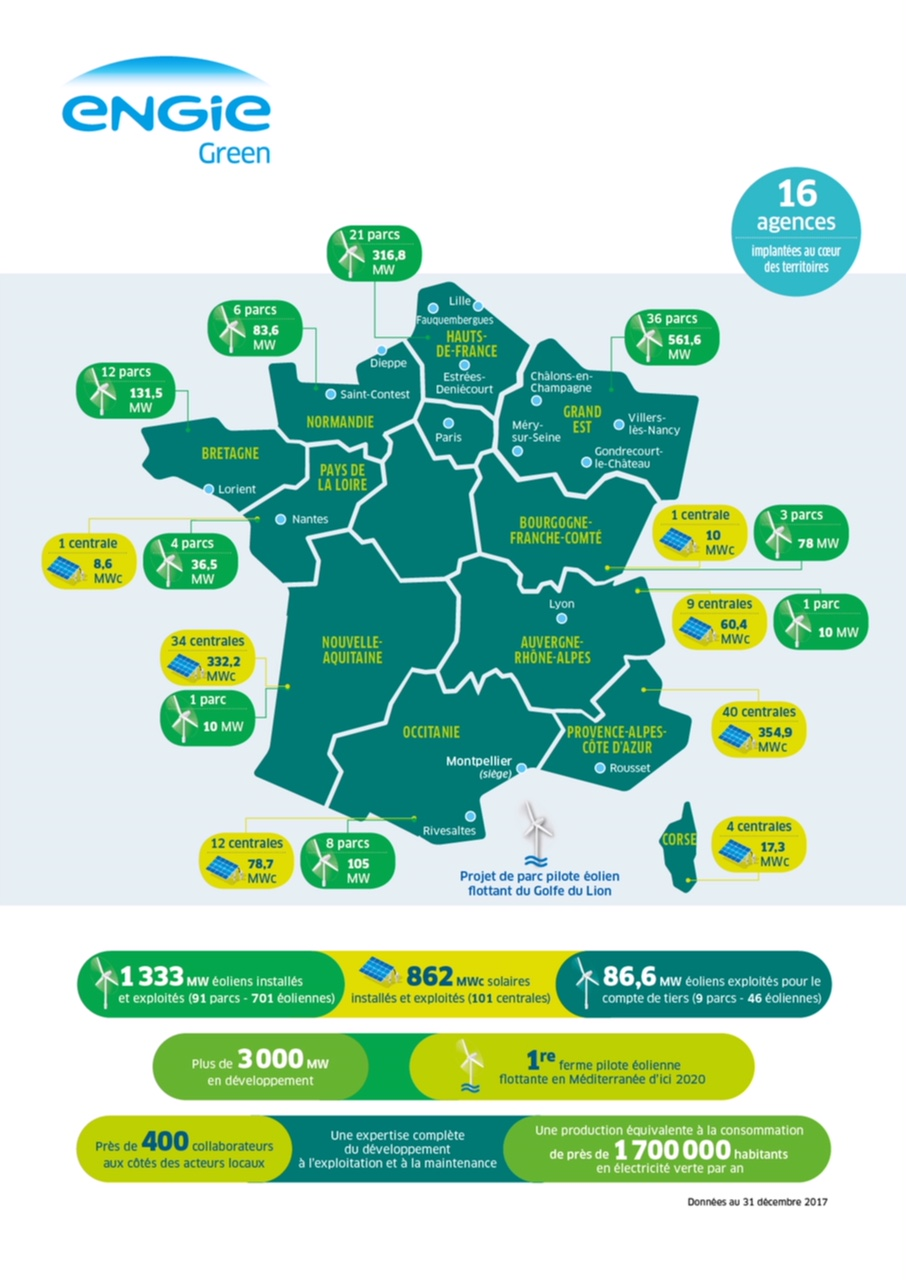
\includegraphics[scale=0.5]{rapport/images/Ch1_infog_engiegreen_2017.jpg} \end{center}
\caption{Infographie Engie 2018}
\end{figure}

Le projet fil rouge s'inscrit dans le cadre du projet Engie Darwin, qui consiste à connecter 100\% des unités de productions éoliennes et solaires afin de proposer des nouvelles solutions numériques et maximiser la valeur des installations. Pour les équipes de data scientists du projet, il s'agit de mettre à disposition des exploitants des informations valorisées en temps réel sur le parc de production. L'objectif étant notamment d'anticiper les problèmes de maintenance et d'adapter la production à la demande.

\section{Données à notre disposition}
Ce projet fil rouge de data science concerne plus précisément les données issues de la ferme solaire de Blond en Haute-Vienne (Nouvelle-Aquitaine).

\begin{figure}[!ht]
\begin{center}
\includegraphics[scale=0.15]{rapport/images/Ch1_FermeSolaire.png}
\end{center}
\caption{La ferme solaire de Blond}
\end{figure}
\FloatBarrier

Cette installation compte près de 25 000 panneaux photo-voltaïques dont le courant électrique produit est agrégé dans des array box, puis des onduleurs avant d'être transformé pour rejoindre le réseau de distribution.

\begin{figure}[!ht]
\begin{center}
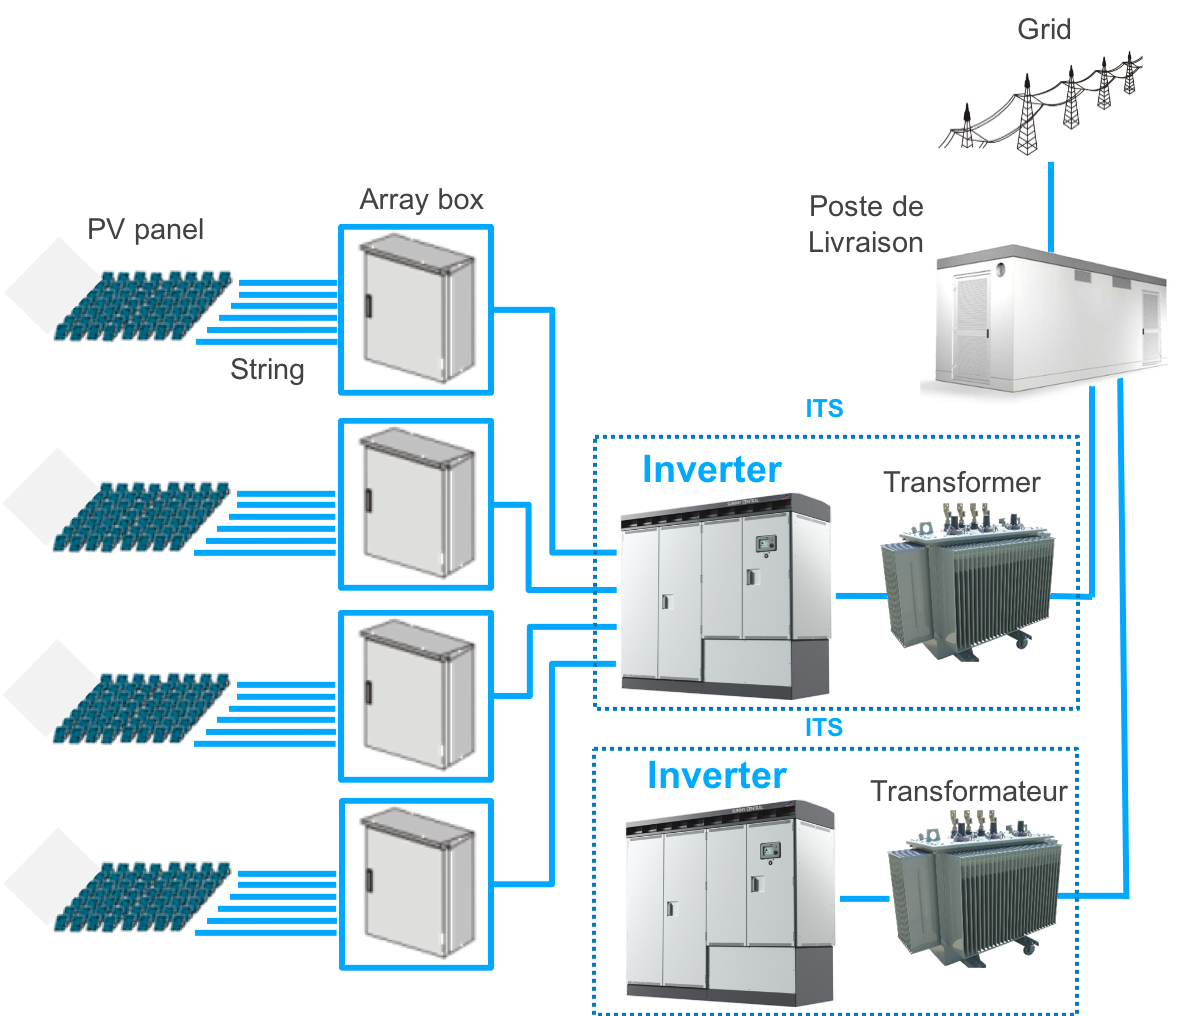
\includegraphics[scale=0.4]{rapport/images/Ch1_Onduleurs.png}
\end{center}
\caption{Schéma de l'installation et des onduleurs}
\end{figure}
\FloatBarrier

Les données mises à notre disposition sont de natures différentes :
\begin{itemize}
\item \textbf{Des données de production électrique} en provenance des 8 onduleurs de la ferme, au pas de temps minute. Ces données brutes sont également accompagnées de données prédites issues de 2 modèles réalisés par l'équipe de Paul Poncet.
\item \textbf{Des données météorologiques} mesurées par une station indépendante et comprenant l'irradiance, température, pluviométrie, hygrométrie et vitesse du vent.
\item \textbf{Des données de maintenance} des équipements sous la forme de journal des événements et des interventions sur la ferme.
\end{itemize}
\paragraph{}
\paragraph{}
\paragraph{}
\section{Problématique et objectifs}
À partir des données précédentes, et en particulier des signaux électriques en provenance des panneaux solaires, il s’agit de \textbf{détecter les sous-performances des équipements en analysant les empreintes des différentes perturbations}.  Les "perturbations" ne sont pas nécessairement des anomalies, mais reflètent des facteurs impactant la production, parmi lesquels on peut citer :

\begin{itemize}
\item \textbf{Les effets saisonniers} : la pousse de la végétation par exemple
\item \textbf{Les ombrages} : ombres portées des lignes montagneuses, la végétation, des ouvrages alentours, etc.
\item \textbf{Les déconnexion d’équipements} : ce sont des pertes de lignes ou de strings qui constituent une réelle anomalie de fonctionnement.
\item \textbf{La température des panneaux} : plus la température est élevée, plus l'efficacité des panneaux diminue.
\item \textbf{Les tendances lentes} : la dégradation progressive liée à la perte de rendement des panneaux, par exemple.
\item \textbf{Les salissures / encrassements} : en particulier dans certains pays avec du sable ou de la poussière où les sites sont exposés aux vents. Dans ce cas l'encrassement tend à croître régulièrement jusqu'à ce qu'une forte averse de pluie vienne nettoyer les panneaux. \cite{JavedW}
\end{itemize}

\begin{figure}[!ht]
\begin{center}
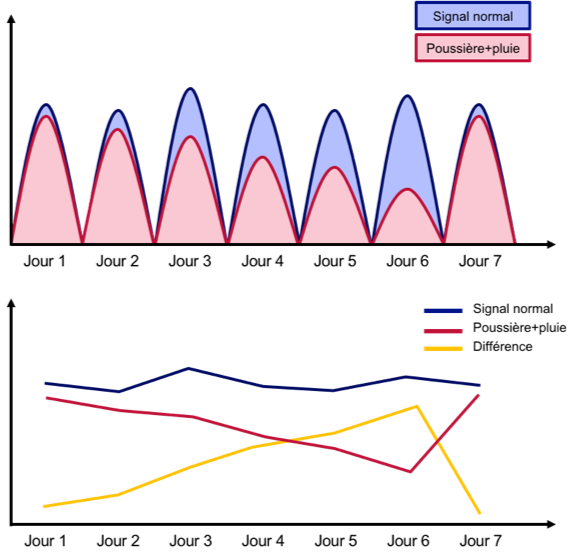
\includegraphics[scale=0.8]{rapport/images/Ch1_SchemaEncrassement.png}
\end{center}
\caption{Schéma du phénomène d'encrassement}
\end{figure}
\FloatBarrier

Dans un contexte de production, l'information de ces sous-performance et la détection des anomalies avérées seraient transmises à l’exploitant pour action.

\section{Approche proposée par Engie}
Outre nos recherches bibliographiques, deux approches nous ont été suggérées pour traiter le problème :
\begin{enumerate}
\item \textbf{Une approche globale} visant à retrouver les effets de façon simultanée et à définir ce que serait le signal normal.
\item  \textbf{Une approche par décomposition du signal par onduleur}, basée les résidus issus de la différence entre les données brutes et les modèles créés par Engie. L'utilisation d'une décomposition par ondelettes a été suggérée pour retrouver les signatures typiques du signal.
\end{enumerate}
%\let\clearpage\relax

\chapter{Description des données}


\section{Influence du rayonnement solaire sur la production électrique}



\section{Différents modèles de production électriques}


\section{}




\chapter{Détection d'anomalie}

\section{Présentation générale des différentes méthodes}
\subsection{Types d'anomalies}
La détection d'anomalie dans les données est une méthode consistant à trouver des motifs non 
usuels dans la donnée. Ces anomalies sont différentes du bruit existant dans les données.
Il existe différent types d'anomalies:
\begin{enumerate}
\item Les anomalies ponctuelles (un point dont la valeur excède la gamme de valeur de la distribution des données)
\item Les anomalies contextuelles (des valeurs non usuels pour le contexte donné)
\item Les anomalies collectives (une gamme de valeur non usuels)
\end{enumerate}

\paragraph{}
Dans le cas où on suppose que les données sont paramétriques, on suppose
que les données normales suivent une loi gaussienne.
Les anomalies sont les données qui ne suivent pas cette distribution.

L'anormalité est caractérisée par la distance de Mahalanobis
\begin{equation}
d(x,y) = \sqrt{(x-y)^\top \Sigma (x-y)} 
\end{equation}
\paragraph{}
Si on ne suppose rien sur la loi que suit les données normales, d'autres méthodes sont utilisées comme 

\begin{enumerate}
\item Density based
\item Distance based
\end{enumerate}

\subsubsection{Random forest}
On définira une notion de similarité et de distance entre les données .

La similarité entre les 2 observation est basé sur le nombre de fois les 2 observations
correspondent à la même feuille. 
\begin{equation}
prox(n,k)= \frac{similarity}{number tree}
\end{equation}
Les anomalies correspondent aux observations qui ont une petite pro par rapport aux autres observations 

%\subsubsection{Contextual anomalies}
\subsection{Isolation Forest}
Un arbre est construit pour détecter l'anomalie




\subsection{LOF (Local Outlier Factor)}
Identifier la densité local de chaque point et la comparer avec les voisins.
The local reachibility factor density is computed as

\begin{equation}
density  = ..
\end{equation}
\paragraph{}


\subsection{1 class SVM}


\subsection{L'algorithme du LSTM}

\subsection{Extraction des coefficients des ondelettes à utiliser comme feature}
Les données peuvent être projetés dans une autre base pour pouvoir détecter le comportement normal et anormal.
Dans le cas des séries temporelles, on utilise souvent une base composée des coefficients d'ondelettes.

%Il existe une littérature assez conséquente sur la détection d'anomalie pour les maladies cardiaques. Dans ce domaine, on utili


\begin{thebibliography}{1}
\bibitem{Breiman}
BREIMAN, Leo. 
\emph{Random forests.}
Machine learning, 2001, vol. 45, no 1, p. 5-32.

\bibitem{BreunigM}
	 BREUNIG, Markus M., KRIEGEL, Hans-Peter, NG, Raymond T., et al. 
	 \emph{LOF: identifying density-based local outliers.} 
	 In : ACM sigmod record. ACM, 2000. p. 93-104.
	  
\bibitem{ChandolaV}	  
	  CHANDOLA, Varun, BANERJEE, Arindam, et KUMAR, Vipin. 
	  \emph{Anomaly detection: A survey.}
	   ACM computing surveys (CSUR), 2009, vol. 41, no 3, p. 15.
	   
\bibitem{MalhotraP}	  
	MALHOTRA, Pankaj, VIG, Lovekesh, SHROFF, Gautam, et al.
	\emph{Long short term memory networks for anomaly detection in time series.} 
	In : Proceedings. Presses universitaires de Louvain, 2015. p. 89.
	   
\bibitem{KeohgE}    
   KEOGH, Eamonn, LONARDI, Stefano, et CHIU, Bill'Yuan-chi'. 
   \emph{Finding surprising patterns in a time series database in linear time and space.} In : Proceedings of the eighth ACM SIGKDD international conference on Knowledge discovery and data mining. ACM, 2002. p. 550-556.
	   
\bibitem{LiZ} 	
Li, Z., Li, Z., Yu, N., Wen, S. 	   
	   \emph{Locality-Based Visual Outlier Detection Algorithm for Time Series}
	   Security and Communication Networks, 2017.  
\bibitem{ChenC} 	   
	Chen, C., Liu, L. M. (1993).
\emph{Joint estimation of model parameters and outlier effects in time series.}
Journal of the American Statistical Association, 88(421), 284-297.	   

\bibitem{DingH} 	
DING, Hui, TRAJCEVSKI, Goce, SCHEUERMANN, Peter, et al. 
\emph{Querying and mining of time series data: experimental comparison of representations and distance measures.}
 Proceedings of the VLDB Endowment, 2008, vol. 1, no 2, p. 1542-1552.	
	

	
	   
\end{thebibliography}



\chapter{Decomposition en ondelettes}



\section{Principe}
\paragraph{}
Pour le traitement du signal, différentes méthodes de décomposition existent.
La plus connue et utilisée, est la transformée de Fourier. Cette dernière permet de filtrer le signal à différentes fréquences temporelles. Elle informe donc sur le contenu fréquentiel du signal.
\paragraph{}
Elle possède une limitation majeure dans la connaissance du comportement local d'une fonction.
Ce défaut a été observé par D.Gabor qui a réussi à pallier à cette inconvénient en utilisant la STFT (short-time Fourier transform). Seulement la résolution temporelle restait insuffisante.
Elle n'est donc pas adéquate pour l'étude de signaux dans un régime transitoire. ~\cite{GaoR}
\paragraph{}
La décomposition en ondelettes permet de pallier à ce défaut.
Elle prend en compte la variabilité fréquentielle de la fonction. 
Elle donne donc une \emph{représentation temps-fréquence d'un signal} ~\cite{JBigot}.
et permet donc de fournir une localisation temporelle.

\subsection{Définition}
La transformée en ondelettes ~\cite{JBigot} continue d'une fonction $f  \in L^{2}(\R)$ au point $x \in \R $
et à l'échelle $ s>0 $ est définie par  :
\begin{equation}
W_{f}(x,s) = <f,\Psi_{x,s}> = \int^{+\infty}_{- \infty} \frac{1}{\sqrt{s}}f(t)\Psi(\frac{t-x}{s})dt
\end{equation} 
Une transformée en ondelettes peut s'écrire sous la forme d'un filtrage par convolution :
\begin{equation}
W_{f}(x,s) = f * \psi^{*}_{s}(x)
\end{equation}
avec  $\psi^{*}_{s}(x) = \frac{1}{\sqrt{s}} \psi(\frac{-t}{s})$

\paragraph{}
La transformée en ondelette satisfait les propriétés de conservation de l'énergie du signal.



\paragraph{}
L'ondelette choisie doit avoir :
\begin{enumerate}
\item un support compact pour obtenir une localisation dans l'espace
\item une moyenne égale à 0


\end{enumerate}
propriété:
 orthogonalité, lissante
\paragraph{}
Il existe plusieurs types d'ondelettes :
\begin{enumerate}
\item Haar
\item Mexican hat
\item Morlet
\item Daubechie

\end{enumerate}

On utilisera l'ondelette Daubechie qui est la plus souvent utilisée d'après la littérature.

\paragraph{}
La transformée en ondelette permet de représenter une fonction comme une combinaison linéaire de fonctions de bases d'ondelettes.

Elle permet de réprésenter une fonction dans une \emph{représentation multirésolution d'ondelettes}. Celà consiste à une séquences d'espaces fermées $V_{m}$ de $ L^{2}(\R)$ où
$L^{2}(\R)$ est un espace d'Hilbert de outes les fonctions au carré intégrables.
Ces espaces caractérisent le comportement d'une fonction à l'échelle $2^{m}$ échantillons par unité de longueurs.


\paragraph{}
Les coefficients de la transformée en ondelettes sont calculées par
\begin{equation}
W_{f}(x,s) = f * \psi^{*}_{s}(x)
\end{equation}

\section{Méthodologie}

\subsection{Decomposition}
La fonction que l'on souhaite décomposer est réalisée de la façon suivante :
\begin{equation}
f(x)= \sum^{2j0-1}_{k=0} \alpha_{0,k}\phi_{j0,k} +\sum \sum^{2j0-1}_{k=0}\beta_{j,k}\psi_{j,k}
\end{equation}
%\alpha_{0,k}\phi_{j0,k} +\sum \sum^{2j0-1}_{k=0}\beta_{j,k}\psi_{j,k}
\begin{equation}
f(x) =f_{J0}(x) +\sum_{j>j0} D_{j}(x)
\end{equation}

Les coefficients d'ondelettes sont calculées de la manière suivante :
avec le coefficient d'échelle :
\begin{equation}
\alpha = \int^{1}_{0}f(x)\phi(x)dx
\end{equation}
et le coefficient de détail :
\begin{equation}
\beta_{j,k} = \int^{1}_{0}f(x)\psi(x)dx
\end{equation}

$phi(x)$ est appelé l'ondelette mère
et $\psi(x) $ est l'ondelette père .

Pour une ondelette de Haar (ou Daubechie) , elles sont de la forme 



\begin{equation}
\psi(x) = \left\{
    \begin{array}{ll}
        -1 & \mbox{si } \{x\} \in [0,1/2] \\
        1 & \mbox{si } \{x\} \in ]1/2,1]
    \end{array}
\right.
\end{equation}


\begin{equation}
\phi(x) = \left\{
    \begin{array}{ll}
        1 & \mbox{si } \{x\} \in [0,1[ \\
        0 & \mbox{sinon.} 
     \end{array}
\right.
\end{equation}



\paragraph{}
Débruitage par seuillage
\subsection{Détection d'anomalie à l'aide des coefficients dans la base en ondelettes}
Pour détecter les anomalies, on se concentrera sur la projection des données sur la base formée des coefficients d'ondelettes.
\section{Résultat}


\begin{thebibliography}{1}
\bibitem{StMallat}
	  Stéphane Mallat,
	  \emph{A Wavelet Tour of Signal Processing}.
	  Elsevier, 
	  1999.
	  
\bibitem{JBigot}
	Jérémie Bigot,
	\emph{Analyse par ondelettes}
	Université Paul Sabatier,
	2009		  
\bibitem{AGraps}
	Amara Graps
	\emph{An Introduction to Wavelets}
	 IEEE computational science and engineering, 1995, vol. 2, no 2, p. 50-61,
	 1995.
\bibitem{Cchui}
		Charles K Chui
      	\emph{An Introduction to Wavelets}
      	 Elsevier, 2016.
\bibitem{GRama}
	GENÇAY, Ramazan, SELÇUK, Faruk, et WHITCHER, Brandon J
	 \emph{An introduction to wavelets and other filtering methods in finance and economics} 			      Elsevier, 2001.
\bibitem{WojPrz} 
  WOJTASZCZYK, Przemyslaw. 
  \emph{A mathematical introduction to wavelets.}
   Cambridge University Press, 1997.
\bibitem{GStrang}  
	STRANG, Gilbert et NGUYEN, Truong.
	\emph{Wavelets and filter banks.}
	 SIAM, 1996.
\bibitem{SMalla92} 	 
MALLAT, Stephane et HWANG, Wen Liang.
\emph{Singularity detection and processing with wavelets. IEEE transactions on information theory} X vol. 38, no 2, p. 617-643, 1992.   

\bibitem{GaoR}  
Gao, R. X., Yan, R. (2010)
\emph{Wavelets: Theory and applications for manufacturing.} 
Springer Science \& Business Media.   
%   
\bibitem{Guler}
GULER, Inan et UBEYLI, Elif Derya
\emph{ECG beat classifier designed by combined neural network model.}
 Pattern recognition, 2005, vol. 38, no 2, p. 199-208.
\bibitem{INCE}
INCE, Turker, KIRANYAZ, Serkan, et GABBOUJ, Moncef.
\emph{A generic and robust system for automated patient-specific classification of ECG signals.} IEEE Transactions on Biomedical Engineering, 2009, vol. 56, no 5, p. 1415-1426.

\end{thebibliography}
%\chapter{Description des données}

Les données proviennent du parc photo-voltaïque de Blond, géré par Solaire Direct une filiale d'Engie.
Elles sont groupées en trois catégories:
\begin{itemize}
\item Données électriques au pas de temps minute représentant la production électrique brute et modélisée par Engie
\item Données météo comme l'irradiance, la température, la pluviométrie, la hygrométrie et la vitesse du vent
\item Données de maintenance des équipements
\end{itemize}

Ces données alimentent une base de donnée SQL Server nommée « Agrégation / Reporting ».
Engie procède à l'extraction de l'ensemble des données depuis la base SQL et met à disposition de l'équipe Télécom Paristech un lot de fichiers plats au format csv.

La liste des fichiers plats csv reçus est la suivante:
\begin{itemize}
\item PV.csv
\item INVERTER.csv
\item ITS.csv
\item PLANT.csv
\item PCI.csv
\item architecture.xlsx
\item WEATHER\_STATION\_DATA\_SETS.csv
\item EVENT.csv
\end{itemize}

L'ensemble des fichiers contient des données brutes sur 18 mois, excepté le fichier PV.csv qui contient des données déjà formatées et nettoyées sur 5 mois.
Pour le moment, ce sont les données provenant de ce fichier qui sont utilisées.


\section{Données formatées/nettoyées}

Ces données formatées/nettoyées sont fournies au niveau du fichier « PV.csv ». Elles sont échantillonnées dans le temps avec un pas de 10 minutes et contiennent des informations sur l'irradiance, sur la puissance produite et agrégée au niveau de l'onduleur(inverter en anglais).
Nous avons 8 onduleurs différents.

En plus de la puissance produite et de l'irradiance nous avons deux colonnes supplémentaires concernant la puissance prédite par deux modèles différents créés par Engie.
La puissance prédite dans la colonne « Pred\_self » provient d'un modèle qui prend en compte les données électriques ainsi que les divers données météo. 
La puissance prédite dans la colonne « Pred\_neighbour » provient d'un modèle qui prend en compte la puissance produite par les onduleurs voisins. 

\begin{figure}[!ht]
\begin{center} 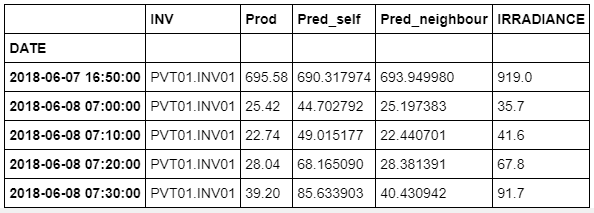
\includegraphics[scale=0.8]{rapport/images/Ch51_PV_head.png} \end{center}
\caption{Extrait du fichier PV.csv}
\end{figure}

\newpage
\section{Données brutes}
\subsection{Les données électriques}

Les données électriques sont collectées au niveau de chaque onduleur, mais elles sont également agrégées à plusieurs niveaux jusqu'à la ferme solaire entière. 

La structure de la ferme solaire est constituée de différents équipements, avec les feuilles représentant les onduleurs (INV), ensuite les transformateurs (ITS), les antennes (FEEDER) et l'entité qui représente la ferme solaire (PLANT).

\begin{figure}[!ht]
\begin{center} 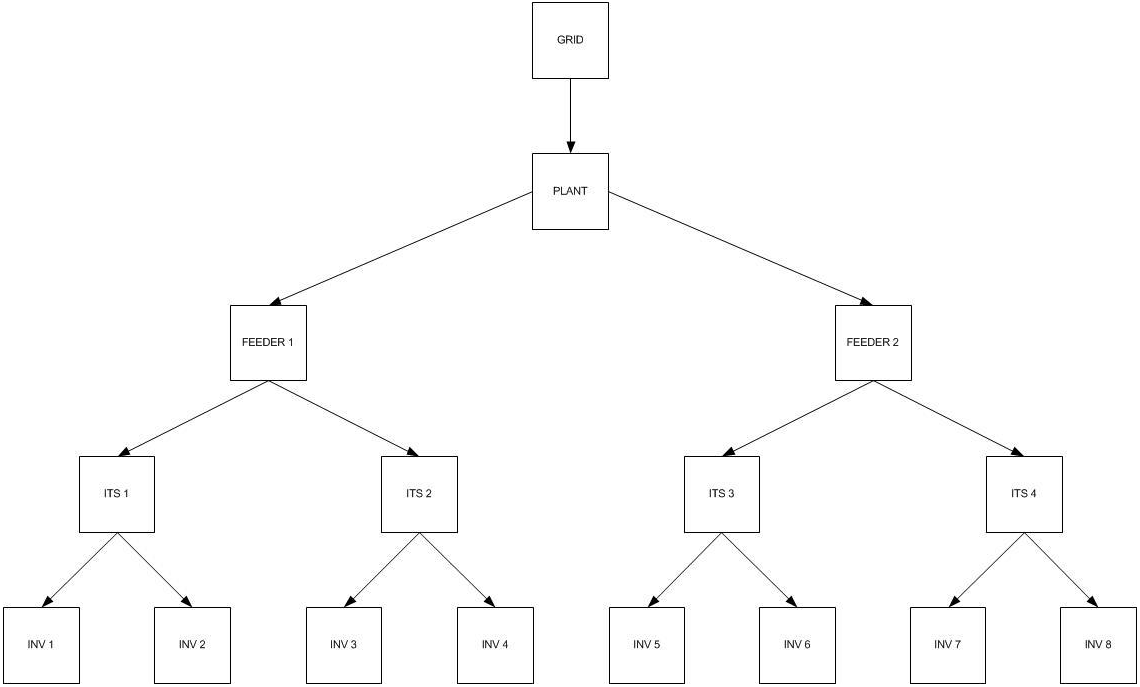
\includegraphics[scale=0.5]{rapport/images/Ch51_equipements_parc.png} \end{center}
\caption{Équipements de la ferme solaire}
\end{figure}

\newpage

Le fichier « INVERTER.csv » contient les mesures effectuées toutes les minutes du voltage, de l'intensité du courant, de la résistance d’isolement, de la température interne, de la puissance active, de la puissance réactive ainsi que de la puissance active produite depuis la mise en service.

\begin{table}[htb]
\resizebox{15cm}{!}{
\begin{center}
   \begin{tabular}{ || l | l|| }
     \hline
     \rowcolor{lightgray} \ \  Nom de la colonne & Description \\ \hline
     DATE & La date à laquelle les mesures ont été effectuées \\ \hline
     INVERTER\_ID & L'identifient de l'onduleur \\ \hline
     DC\_VOLTAGE & U DC, V \\ \hline
     AC\_VOLTAGE\_U12 & U12, V \\ \hline
     AC\_VOLTAGE\_U23 & U23, V \\ \hline
     AC\_VOLTAGE\_U31 & U31, V \\ \hline
     DC\_CURRENT & I DC, A \\ \hline
     AC\_CURRENT\_I12 & I12, A \\ \hline
     AC\_CURRENT\_I23 & I23, A \\ \hline
     AC\_CURRENT\_I31 & I31, A \\ \hline
     INSULATION\_RESISTANCE  & Résistance d’isolement \\ \hline
     INTERNAL\_TEMPERATURE\_1 & Température interne 1, \degree C \\ \hline
     INTERNAL\_TEMPERATURE\_2 & Température interne 2, \degree C \\ \hline
     INTERNAL\_TEMPERATURE\_3 & Température interne 3, \degree C \\ \hline
     ACTIVE\_POWER & P, kW \\ \hline
     REACTIVE\_POWER & Q, kVAr \\ \hline
     COMMISSIONING\_ACCUMULATED\_ACTIVE\_ETU & Comptage d'énergie active produite depuis MES, kWh \\ 
     \hline
   \end{tabular}
 \end{center}}
\caption{La structure du fichier INVERTER.csv }
\end{table}

Le fichier « ITS.csv » regroupe des mesures de températures et d'irradiance au niveau des transformateurs qui regroupent deux onduleurs. Ces mesures sont réalisées tous les 10 minutes.

\begin{table}[htb]
\resizebox{15cm}{!}{
\begin{center}
   \begin{tabular}{ || l | l|| }
     \hline
     \rowcolor{lightgray} \ \  Nom de la colonne & Description \\ \hline
     DATE & La date à laquelle les mesures ont été effectuées  \\ \hline
     ITS\_ID  & Identifiant de l’ITS associé  \\ \hline
     GT\_IRRADIANCE &  Irradiance POA, W/{\SI{}{\metre\squared}} \\ \hline
     MODULE\_TEMPERATURE  & Température sous module, \degree C \\ \hline
     SHELTER\_HV\_TEMPERATURE  & Température local HT, \degree C \\ \hline
     SHELTER\_LV\_TEMPERATURE  & Température local BT, \degree C \\
     \hline
   \end{tabular}
 \end{center}}
\caption{La structure du fichier ITS.csv }
\end{table}

\newpage

Le fichier « PLANT.csv » contient les mesures électriques agrégées toutes les minutes au niveau de la ferme solaire entière.

\begin{table}[htb]
\resizebox{15cm}{!}{
\begin{center}
   \begin{tabular}{ || l | l|| }
     \hline
     \rowcolor{lightgray} \ \  Nom de la colonne & Description \\ \hline
     DATE & La date à laquelle les mesures ont été effectuées \\ \hline
     PLANT\_ID & Identifiant du parc \\ \hline
     DAILY\_ACCUMULATED\_GT\_IRRADIANCE & Cumul irradiance POA journalier, Wh/{\SI{}{\metre\squared}} \\ \hline
     REF\_IRRADIANCE & Irradiance de Référence, W/{\SI{}{\metre\squared}} \\ \hline
     ACTIVE\_POWER\_CONSUMED & Puissance active consommée, kW \\ \hline
     REACTIVE\_POWER\_CONSUMED & Puissance réactive consommée, kVAr \\ \hline
     U12\_AUX\_ELEC\_METER & U12, V \\ \hline
     U23\_AUX\_ELEC\_METER & U23, V \\ \hline
     U31\_AUX\_ELEC\_METER & U31, V \\ \hline
     INSTANT\_ACTIVE\_POWER & Puissance active instantanée, kW \\ \hline
     INSTANT\_REACTIVE\_POWER & Puissance réactive instantanée, kVAr \\ \hline
     COMMISSIONING\_ACCUMULATED\_ACTIVE\_EFU & Comptage d'énergie active consommée depuis MES, kWh \\ \hline
     COMMISSIONING\_ACCUMULATED\_ACTIVE\_ETU & Comptage d'énergie active produite depuis MES, kWh \\ \hline
     COMMISSIONING\_ACCUMULATED\_REACTIVE\_EFU & Comptage d’énergie réactive consommée depuis MES, kVArh \\ \hline
     COMMISSIONING\_ACCUMULATED\_REACTIVE\_ETU & Comptage d'énergie réactive produite depuis MES, kVArh \\ \hline
     DAILY\_ACCUMULATED\_ACTIVE\_EFU & Comptage journalier d'énergie active consommée, kWh \\ \hline
     DAILY\_ACCUMULATED\_ACTIVE\_ETU & Comptage journalier d'énergie active produite, kWh \\ \hline
     DAILY\_ACCUMULATED\_REACTIVE\_EFU & Comptage journalier d’énergie réactive consommée, kVArh \\ \hline	 
     DAILY\_ACCUMULATED\_REACTIVE\_ETU & Comptage journalier d'énergie réactive produite, kVArh \\ \hline	 
     U12\_SD\_ELEC\_METER & U12, V \\ \hline	 
     U23\_SD\_ELEC\_METER & U23, V \\ \hline	 
     U31\_SD\_ELEC\_METER & U31, V \\
     \hline
   \end{tabular}
 \end{center}}
\caption{La structure du fichier PLANT.csv }
\end{table}

Le fichier « PCI.csv » fournit la puissance crête installée à plusieurs niveaux d'agrégation à partir des boîtiers de raccordement jusqu'à la ferme solaire entière. Les données contenues dans ce fichier ne sont pas temporelles. 

\begin{table}[htb]
{\fontsize{6}{8} \selectfont 
\resizebox{15cm}{!}{
\begin{center}
   \begin{tabular}{ || l | l|| }
     \hline
     \rowcolor{lightgray} \ \  Nom de la colonne & Description \\ \hline
     P\_ID & Identifiant de la ferme solaire  \\ \hline
     P\_NAME & Nom de la ferme solaire  \\ \hline
     P\_PCI & Puissance crête installée de la ferme solaire \\ \hline
     F\_ID & Identifiant de l'antenne \\ \hline
     F\_NAME & Nom de l'antenne \\ \hline
     F\_PCI & Puissance crête installée de l'antenne \\ \hline
     ITS\_ID & Identifiant du transformateur \\ \hline
     ITS\_NAME & Nom du transformateur \\ \hline
     ITS\_PCI & Puissance crête installée du transformateur \\ \hline
     INV\_ID & Identifiant de l'onduleur \\ \hline
     INV\_NAME & Nom de l'onduleur \\ \hline
     INV\_PCI & Puissance crête installée de l'onduleur \\ \hline
     AB\_ID & Identifiant du boîtier de raccordement(array box) \\ \hline
     AB\_NAME & Nom du boîtier de raccordement(array box) \\ \hline
     AB\_PCI & Puissance crête installée boîtier de raccordement(array box) \\	 
     \hline
   \end{tabular}
 \end{center}}}
\caption{La structure du fichier PCI.csv }
\end{table}

\newpage

Le fichier « architecture.xlsx » contient la table de correspondance entre les identifiants et les noms des différents composants de la ferme solaire. 

\begin{table}[htb]
\resizebox{15cm}{!}{
\begin{center}
   \begin{tabular}{ || l | l|| }
     \hline
     \rowcolor{lightgray} \ \  Nom de la colonne & Description \\ \hline
     ETL\_ID & Identifiant de l'extracteur ETL \\ \hline
	 ETL\_NAME & Type de l'extracteur (temps réel ou différé) \\ \hline
     PLANT\_ID & Identifiant de la ferme solaire \\ \hline
     PLANT\_NAME & Nom de la ferme solaire \\ \hline
     WEATHER\_STATION\_ID & Identifiant de la station météo \\ \hline
     WEATHER\_STATION\_NAME & Nom de la station météo \\ \hline
     FEEDER\_ID & Identifiant de l'antenne \\ \hline
     FEEDER\_NAME & Nom de l'antenne \\ \hline
     ITS\_ID & Identifiant du transformateur \\ \hline
     ITS\_NAME & Nom du transformateur \\ \hline
	 INVERTER\_ID & Identifiant de l'onduleur \\ \hline
     INVERTER\_NAME & Nom de l'onduleur \\ \hline
     ARRAY\_BOX\_ID & Identifiant du boîtier de raccordement(array box) \\ \hline
     ARRAY\_BOX\_NAME & Nom du boîtier de raccordement(array box) \\
     \hline
   \end{tabular}
 \end{center}}
\caption{La structure du fichier architecture.xlsx }
\end{table}

\subsection{Les données météo}

Les données météo en dehors de la température se retrouvent au niveau du fichier « WEATHER\_STATION\_DATA\_SETS.csv ». Il contient les valeurs de l'irradiance, de la température, de la pluviométrie, de la hygrométrie et de la vitesse du vent. La température et l'irradiance sont collectées tous les minutes, alors que la pluviométrie, la hygrométrie et la vitesse du vent sont enregistrées tous les 10 minutes seulement.

\begin{table}[htb]
\resizebox{15cm}{!}{
\begin{center}
   \begin{tabular}{ || l | l|| }
     \hline
     \rowcolor{lightgray} \ \  Nom de la colonne & Description \\ \hline
     DATE & Horodate associée aux valeurs \\ \hline
	 WEATHER\_STATION\_ID & Identifiant de la station météo associée \\ \hline
     HYGROMETRY & Hygrométrie, \\ \hline
     GH\_IRRADIANCE & Irradiance GHI, W/{\SI{}{\metre\squared}} \\ \hline
     PLUVIOMETRY & Pluviométrie, mm \\ \hline
     GT\_IRRADIANCE & Irradiance GT station météo, W/{\SI{}{\metre\squared}} \\ \hline
     AMBIENT\_TEMPERATURE & Température ambiante extérieure, \degree C \\ \hline
     WIND\_SPEED & Vitesse du vent, m/s \\
     \hline
   \end{tabular}
 \end{center}}
\caption{La structure du fichier WEATHER\_STATION\_DATA\_SETS.csv }
\end{table}

\subsection{Données de maintenance des équipements}

Les données contenues dans le fichier « EVENT.csv » répertorient les différents événements de maintenance des équipements de la ferme solaire, issues du ou des Cahiers Des Incidents déjà existants (conservation de la mémoire des parcs). 
Dans ce fichier nous retrouvons également différentes colonnes contenant le calcul des énergies non distribuées (END) suite à l'événement courant.

\begin{table}[htb]
\resizebox{15cm}{!}{
\begin{center}
   \begin{tabular}{ || l | l|| }
     \hline
     \rowcolor{lightgray} \ \  Nom de la colonne & Description \\ \hline
     ID & Identifiant de l’événement \\ \hline
	 GROUP\_ID & Identifiant du groupe lorsque l’événement fait partie d’un groupe \\ \hline
     NB\_END\_EVENTS\_IN\_GROUP & Nombre d’événements dans un groupe \\ \hline
     STATUS & Etat de l’événement \\ \hline
     START\_DATE & Date de début \\ \hline
     END\_DATE & Date de fin \\ \hline
     TOTAL\_DURATION & Durée de l’événement \\ \hline
     PLANT\_ALIAS & Alias de la ferme solaire \\ \hline
     FEEDER\_ALIAS & Alias de l'antenne \\ \hline
     ITS\_ALIAS & Alias du transformateur \\ \hline
	 INVERTER\_ALIAS & Alias de l'onduleur \\ \hline
     ARRAY\_BOX\_ALIAS & Alias du boîtier de raccordement \\ \hline
     ROOT\_CAUSE & Root cause associée \\ \hline
     ASSIGNMENT\_REPORTING & Description de l’affectation de l’événement \\ \hline
     DESCRIPTION & Description de l’événement \\ \hline
     END\_TOTAL & La valeur de l’END calculée, kWh \\ \hline
     END\_SD & La part Solaire Direct de l’END calculée, kWh \\ \hline
     END\_NOT\_SD & La part non Solaire Direct de l’END calculée, kWh \\ \hline
     FULL\_NAME & Non renseigné \\ \hline
     DELETED\_AT & Date de suppression de l’événement \\ \hline	 
     WITH\_MISSING\_DATA & Booléen indiquant qu’il y a au moins une donnée manquante pour effectuer le calcul de l’END \\	 
     \hline
   \end{tabular}
 \end{center}}
\caption{La structure du fichier EVENT.csv }
\end{table}

La cause ou le type de l'événement est situé au niveau du champ « ROOT\_CAUSE » et peu prendre une des valeurs suivantes :

\begin{itemize}
\item FEEDER\_CIRCUIT\_BREAKER\_OPENED
\item FEEDER\_LOCAL\_CONTROL\_MODE
\item INVERTER ACTIVE POWER NULL
\item INVERTER\_COM\_FAIL
\item INVERTER\_STAND\_BY\_STATUS
\item INVERTER\_STOP\_STATUS
\item ITS\_CIRCUIT\_BREAKER\_OPENED
\item ITS\_LOCAL\_CONTROL\_MODE
\item PLANT ACTIVE POWER LIMITATION VALUE
\item PLANT\_EMERGENCY\_STOP\_REQUEST
\item PLANT\_GRID\_DISCONNECT\_REQUEST
\item PLANT\_GRID\_WAIT\_FOR\_AUTHOR
\item PLANT\_GTE\_TRIP
\item PLANT INSTANT ACTIVE POWER NULL
\item PLANT\_MAIN\_CIRCUIT\_BREAKER\_OPENED
\end{itemize}

Note : à cette date nous attendons encore de confirmer la signification exact de chaque type d'événement afin d'inclure ces informations dans nos jeux de données.
%\chapter{Réalisation du projet}

\section{Préparer les données}
\section{Explorer les données}
\subsection{Premières expérimentations}
Les premières explorations des données formatées sur 5 mois (issues du fichier PV.csv) nous ont permis d'identifier les élements suivants :

\begin{itemize}
\item Les données de production sont fournies par jour entre 6h50 du matin et 17h.
\item Il existe des jours avec des données manquantes
\item Les onduleurs exhibent des profils et des comportements parfois assez différents entre eux. Cette piste sera plus approfondie par la suite.
\item On remarque la très forte corrélation entre l'irradiance et la production électrique des panneaux photo-voltaïques. L'irradiance suit une courbe en cloche avec un pic autour des 13h-14h. La production électrique stagne autour des 900 $Wm^2$ mettant en avant les limites de production des panneaux solaires. 


\begin{figure}[!ht]
\begin{center}
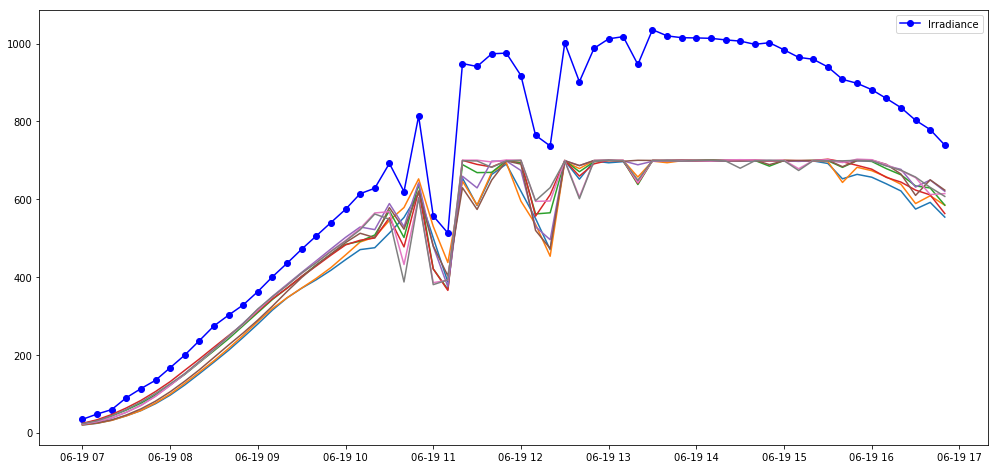
\includegraphics[scale=0.3]{rapport/images/Ch6_Irradiance-Prod.png}
\end{center}
\caption{L'irradiance et la production des 8 onduleurs pour le 19 juin 2018}
\end{figure}
\FloatBarrier
\paragraph{}
\item On peut observer que le modèle prédictif basé sur les données météorologiques est moins précis que son homologue. Il ne tient pas compte du phénomène de plateau contrairement au modèle basé sur les valeurs voisines dont les prédictions sont très précises :

\begin{figure}[h!]
\begin{center}
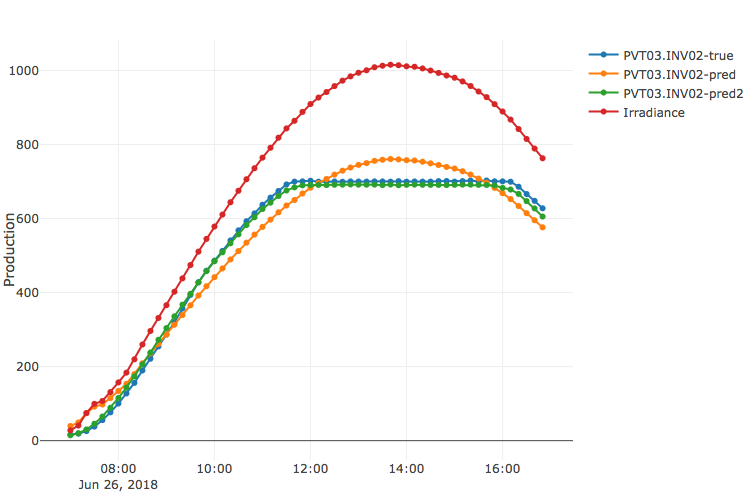
\includegraphics[scale=0.4]{rapport/images/Ch6_26juin.png}
\end{center}
\caption{L'irradiance et la production pour le 26 juin 2018, onduleur PVT03.INV02}
\end{figure}
\FloatBarrier
\item On constate que certaines journées sont très "bruitées" au niveau de l'irradiance, correspondant vraisemblablement à des journées nuageuses ou avec de la pluie, ce que nous tâcherons de mieux comprendre grâce à la décomposition du signal.
\end{itemize}

\section{Décomposer le signal}
\section{Identifier les signatures particulières}
\section{Rechercher les similarités}
\section{Répertorier les anomalies}
\section{Valider la classification}

\appendix
\include{appa}
\include{appb}


\end{document}

